Avant de définir une stratégie de documentation pour le projet Buckless, nous allons
nous intéresser à la manière dont les différents outils présentés précédemment ont été
intégrés par de gros projets open source.\\
Ces projets ont été choisis pour leur similitude avec le projet Buckless, que ce soit
par les technologies utilisées, le type de logiciel produit, l'architecture logicielle
semblable, etc.

\subsection{Nylas N1}
    \subsubsection{Présentation}
        Nylas est une organisation réalisant le projet N1, un client mail se basant sur des technologies web.
        En effet, le projet utilise un chromium\footnote{Navigateur web} embarqué  pour distribuer une application
        web en tant qu'application native. Cela permet d'avoir une interface facilement stylisable et extensible,
        en plus d'être multiplateforme et portable.\\
        Cette interface utilise une API REST, ouverte, dont la documentation est générée à partir du code.
        Malheureusement, le code source de cette API n'est pas disponible et il n'y a pas moyen de connaître la méthode de génération.
        On peut toutefois observer que la génération de la documentation est faite en interne via un script,
        et non automatiquement à l'aide d'intégration continue.

    \subsubsection{Stratégie de documentation}
        \paragraph{}
            Une documentation est aussi disponible pour l'application en elle-même.
            Vu que le projet est basé sur le paradigme de Programation Orienté Objet, les classes sont assez facile à identifier avec "l'API Reference".
            De plus, N1 utilise les Web Components — qui apportent la modularité aux sites webs en découpant chaque partie en composants autonomes,
            et ils sont eux aussi facilement identifiables.

        \begin{figure}[ht]
            \centering
            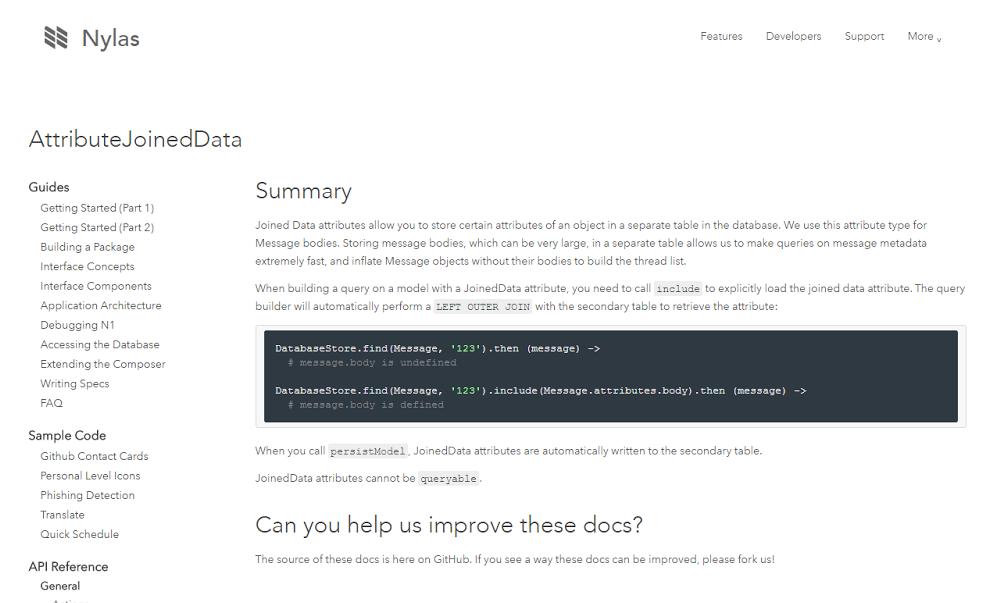
\includegraphics[scale=0.35]{./assets/nylasdoc2.png}
            \caption{Acceuil de la documenation}
        \end{figure}

        \paragraph{}
            L'intérêt majeur de cette documentation est qu'elle est générée via le code source de l'application.
            En utilisant les commentaires, leur script de génération de documentation va créer une arbre syntaxique (AST\footnote{Abstract Syntax Tree}),
            aussi utilisé dans la compilation de programmes.

        \begin{figure}[h]
            \centering
            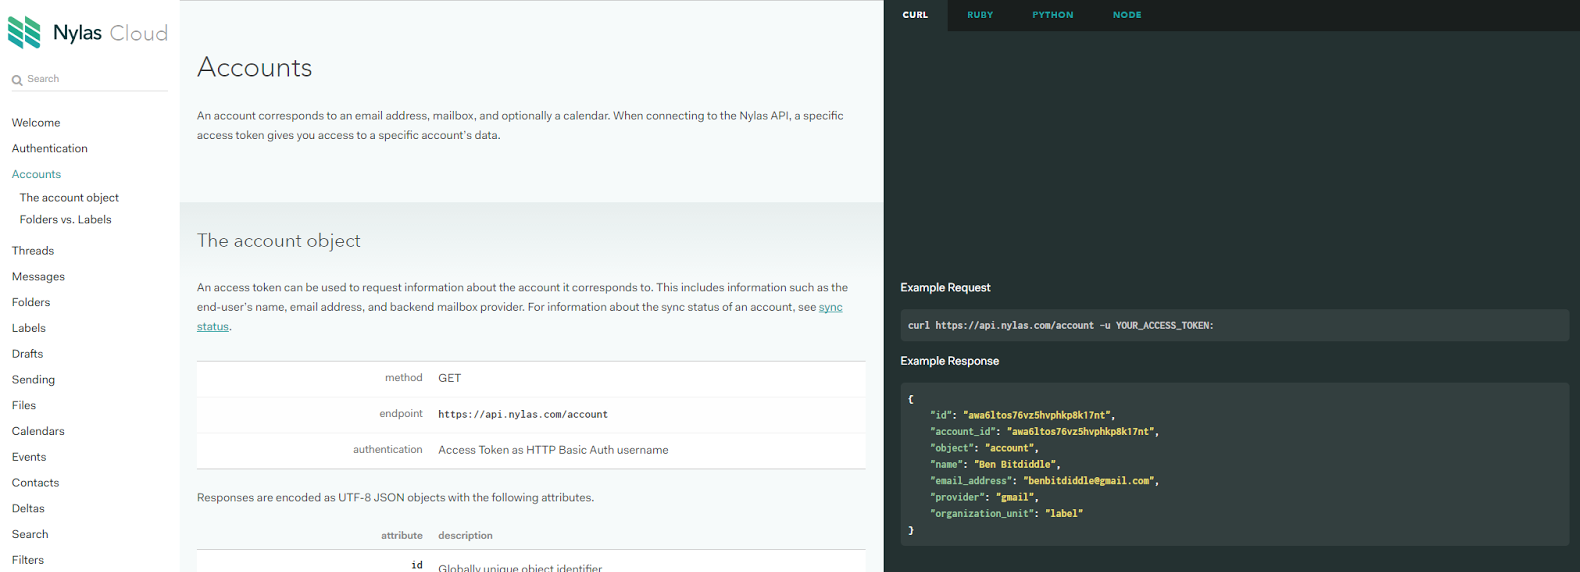
\includegraphics[width=\textwidth]{./assets/nylasdoc.png}
            \caption{La référence de l'API}
        \end{figure}

        \begin{listing}[ht]
            \begin{minted}[
                bgcolor=black,
                fontsize=\footnotesize
            ]{ruby}
# Public: A mutable text container with undo/redo support
class TextBuffer
  @prop2: "bar"

  # Public: Takes an argument and does some stuff.
  #
  # a - A {String}
  # Returns {Boolean}.
  @method2: (a) ->
            \end{minted}
            \caption{Exemple de commentaire TomDoc}
        \end{listing}

        \paragraph{}
            Au niveau des commentaires, un dérivé de jsDoc (TomDoc\cite{tomdoc}) est utilisé, plus adapté
            pour des grosses parties de documentation (là où jsDoc est plus adapté pour l'auto complétion et la documentation rapide).
            La génération de l'AST est faite à l'aide d'une librairie spécialisée\cite{donna}.
        \begin{listing}[ht]
            \begin{minted}[
                bgcolor=black,
                fontsize=\footnotesize
            ]{json}
"files": {
"spec/metadata_templates/classes/class_with_prototype_properties.coffee": {
  "objects": [
        "type": "class",
        "name": "TextBuffer",
        "bindingType": null,
        "classProperties": [],
        "prototypeProperties": [11, 11],
        "doc": " Public: A mutable text container with undo/redo support\n\n "
[...]
            \end{minted}
            \caption{Une partie de l'AST produit sous forme de JSON}
        \end{listing}

        \paragraph{}
            L'AST généré est ensuite transformé en code quasiment exportable en HTML, en utilisant une deuxième librairie\cite{tello}.
            Enfin, Nylas possède un script qui va automatiquement réaliser l'AST puis le contenu et générer le code HTML de la documentation.
            Le code est ensuité publié sur une branche spécifique à la documentation de leur projet.
            Cette branche est automatiquement mise en ligne par GitHub\cite{ghpages} ce qui permet uniquement en
            modifiant le code, de mettre à jour la documentation en ligne directement.